\documentclass[10pt,conference]{IEEEtran}
% If the IEEEtran.cls has not been installed into the LaTeX system files,
% manually specify the path to it:
% \documentclass[conference]{../sty/IEEEtran}
\usepackage{graphicx}
\usepackage{subfigure}
\usepackage{url}
\usepackage{mathtools}
\DeclarePairedDelimiter\ceil{\lceil}{\rceil}
\DeclarePairedDelimiter\floor{\lfloor}{\rfloor}

\begin{document}

% paper title
\title{Identification of black hole states  using matrix based methods: Time series analysis of RXTE satellite data}

% author names and affiliations
% use a multiple column layout for up to three different
% affiliations
%\author{
%\authorblockN{A. Chockalingam}
%\authorblockA{Dept.\ of Electrical Communication Engg.\\
%Indian Institute of Science \\
%Bangalore, 560012, India\\
%Email: spcom2016@gmail.com} \and
%\authorblockN{Rahul Vaze}
%\authorblockA{School of Technology and Computer Science\\
%Tata Institute of Fundamental Research\\
%Mumbai, 400005, India\\
%Email: spcom2016@gmail.com}
%\and
%\authorblockN{Animesh Kumar}
%\authorblockA{Dept.\ of Electrical Engg.\\
%Indian Institute of Technolgy \\
%Bombay, 400076, Mumbai India\\
%Email: spcom2016@gmail.com}
%%\and
%%\authorblockN{Robert Calderbank}
%%\authorblockA{Department of Electrical Engineering\\
%%Princeton University \\
%%Princeton, NJ 08544, USA\\
%%Email: calderbk@math.princeton.edu} \and
%%\authorblockN{Habong Chung}
%%\authorblockA{Department of Electronic\\
%%\& Electrical Engineering\\
%%Hongik University\\
%%Seoul, Korea\\
%%Email: habchung@hongik.ac.kr}
%}
% avoiding spaces at the end of the author lines is not a problem with
% conference papers because we don't use \thanks or \IEEEmembership
% for over three affiliations, or if they all won't fit within the width
% of the page, use this alternative format:
% make the title area
\maketitle

\begin{abstract}
Black hole is one of the fascinating,  however mysterious, astrophysical  objects. In order to identify it one has to look at its environment, often forming a disc-like structure. This disc, called accretion disc, evolves with time transiting from one state to another. For example, in one extreme regime it shows temperature dependent radiations making the disc geometrically thin, and in yet another extreme  regime of time span however radiation turns out to be temperature independent making the disc hot and geometrically thick.  Nevertheless, in general, accretion disc lies in  states intermediate between the two extremes. The present mission is to capture black hole states  explicitly using SVD and PCA based decompositions. In order to do that we rely on time series data of black hole \textit{GRS 1915 + 105} obtained from RXTE satellite. As a black hole cannot be seen directly, identifying its states accurately could help in characterizing its properties. Earlier time series  analysis based on Correlation Integral (CI) approaches, supplemented by theory, argued for four specific states. However there are caveats when data themselves are not free from noise and the  appropriate method for such an analysis itself is exploratory. Present interdisciplinary study aims at, on one hand,  to cross-verify the previous inference, on the other hand to identify, if any,  novel characteristics of black holes. In the experiments conducted it is found that among the proposed matrix based methods, SVD analysis concurs with CI based analysis on all the 12 classes of time series utilized. However, the inference using PCA based approach illustrates that one  class among the 12 turns out to be inconsistent with the other approaches. Investigation into these (in)consistencies  is expected to have long standing implications in astrophysics and otherwise.
\end{abstract}

\section{Introduction}
One of the challenging problems in astrophysics is the understanding of black holes. As a black hole cannot be seen directly, to identify it, one has to look for its environment forming a disc-like structure by the infalling matter called accretion disc. In this work, we focus on the black hole source \textit{GRS 1915+105}, which presents several intriguing facets. It has been classified into 12 different temporal classes: $\alpha$, $\beta$, $\gamma$, $\delta$, $\lambda$, $\kappa$, $\mu$, $\nu$, $\rho$, $\phi$, $\chi$ and $\theta$ \cite{Belloni2000}, with their respective distinct time series. One of the fundamental aspects of the understanding is to determine if the black hole source is a stochastic system or a non-stochastic one. The latter one is related to the well-known turbulent nature of the system. There are several studies that utilize the Correlation Integral (CI) approach to determine the characterization of the black hole data \cite{Mukhopadhyay2004, misra2006}. However, there can also be other approaches to understanding the same data by applying, for e.g.,  matrix-based methods such as Principal Component Analysis (PCA) and Singular Value Decomposition (SVD). It is useful to compare the inferences obtained using these two distinct approaches; the implications of the (dis)similarities in inferences, if any, could lead to questions about understanding the temporal dynamics of the system.

Interestingly, to quantify the properties of a black hole source, along with temporal features one has to look for spectral features as well, they together lead to the true nature of the source. If the source radiation is temperature dependent, it produces more like a blackbody radiation, namely multicolour blackbody or ``diskbb" \cite{Shakura1973}. On the other hand, the temperature independent radiation consists of a power-law tail, named as ``PL" \cite{chakrabarti1995,narayan1994}. While the former leads the underlying accretion disc around the black hole to be geometrically thin, the latter leads to a geometrically thick disc.

In the present study, black hole states are determined by  classifying the given time series, which is photon count rate as a function of time,  as being either stochastic or non-stochastic. This classification is performed using classical matrix based methods, SVD and PCA.
However, the novelty of the study lies in (i) quantifying temporal complexity obtained by SVD decomposition, using topological techniques and (ii) utilizing features derived from PCA for classification. Based on our analysis there are four possible black hole states \cite{Adegoke2018}:
\begin{enumerate}
\item Non-stochastic and diskbb: Keplerian disc \cite{Shakura1973}.
\item Non-stochastic and PL: Advection Dominated Accretion Flow (ADAF)  \cite{narayan1994}.
\item Stochastic and diskbb: Slim disc \cite{Abramowicz1988}.
\item Stochastic and PL: General Advective Accretion Flow (GAAF) \cite{chakrabarti1995, rajesh2010}.
\end{enumerate}

Utility of the proposed approach is illustrated by comparing the results with previously established methods. Following are the major contributions of this paper:
\begin{itemize}
\item SVD decomposition of the data matrix is used for identifying the temporal dynamics of the time series as in \cite{misra2006}. A plot involving the top two right singular vectors of the data matrix shows a clear distinction between stochastic and non-stochastic time series. This distinction is captured using the topological descriptor called Betti numbers \cite{jmlr}. This descriptor for a stochastic time series is topologically simpler than that for a non-stochastic one.

\item PCA, which is a widely used approach for decorrelating features and dimensionality reduction, is utilized for characterizing a time series as stochastic vs non-stochastic. We propose a novel approach by iteratively computing eigenvalue ratios  of covariance matrix for different subintervals of the time series. We  derive multiple features from the eigenvalue ratios and use them to characterize the time series.
\end{itemize}

\section{Related Work}
Several groups have worked on distinguishing between stochastic and non-stochastic time series. The idea of utilizing Permutation Entropy (PE) to determine the complexity measure of a time series was explored in \cite{Bandt2002}. In the work reported in \cite{Boaretto2021}, PE was used to parameterize a given time series  followed by classification using  Neural Network. A Neural Network is trained with noise to learn the parametrization of stochastic signals. The paper explored the idea of utilizing PE of a time series to determine if it is strongly correlated with known stochastic signals (noise).   The claim was that for non-stochastic signals the deviation of the parameter is relatively large as compared to that of the parameter of a stochastic signal.

A different set of reported studies are based on  graph theory and system identification. In the work reported in \cite{lacasa2010}, the authors have utilized the horizontal visibility algorithm in order to distinguish between stochastic and non-stochastic processes. In the approach outlined in \cite{Brunton2016}, the authors combined the idea of sparsity and machine learning with non-linear dynamical systems, in order to determine the governing dynamics. Sparse regression ws used to determine the fewest terms in the equations that govern the dynamics of the phenomenon. The user-defined dictionary of basis functions consists of well-known functions such as polynomials, trigonometric functions and exponentials. The coefficients corresponding to very few of these basis functions will be non-zero for a non-stochastic system. However, the optimal choice of dictionary for a specific choice of problem remains a challenge.

In this work, we propose to utilize classical matrix based methods which do not require any assumptions about the underlying phenomenon.

\section{Proposed Method and Data used}

In this work, we use two different matrix based approaches, one using SVD followed by  Betti number descriptors, and  another using PCA in order to characterize time series as stochastic vs non-stochastic.

\subsection{SVD based approach}
In this approach, we form uncorrelated observation vectors from the raw time series data by utilizing the optimal value of embedding dimension \cite{misra2006}. A data matrix, $D$, is formed with each row  as the  time shifted version of the original time series. The time shift is chosen to be large enough so that each column can be viewed as a different observation vector of the same time evolving phenomenon. Temporal dynamics is understood by utilizing the right singular vectors of the SVD decomposition of $D$ as given in equation (\ref{eqn:svd}) below. Columns of $U$ and $V$  form the left and right singular vectors respectively and $\Sigma$ is a block diagonal matrix with diagonal elements as the singular values, given by
\begin{equation}
D = U \Sigma V^T.
\label{eqn:svd}
\end{equation}
 We observe the plot of the top two right singular vectors (E1 vs E2). For non-stochastic time series this plot is expected to show a specific pattern (attractor behavior, where the plot follows a trajectory leaving a well-defined gap). On the other hand, for stochastic time series, this behavior is absent.

The characteristics of the E1 vs E2 plot are captured using Betti numbers \cite{jmlr}. Betti number descriptor for a $d$-dimensional manifold is a vector of $d$ integers which is represented as $\beta = (\beta_0, \beta_1 \mathellipsis \beta_{d-1})$. Here the E1 vs E2 plots are 2-d manifolds, which are described by  $\beta=(\beta_{0}, \beta_{1}$).  $\beta_{0}$ is the number of blobs (connected components) while $\beta_1$ is the number of $1$-d holes. For a stochastic time series the values of $\beta_{0}$  and $\beta_1$ are expected to be 1 and 0 respectively, as the E1 vs E2 plot consists of one single blob. However for a non-stochastic time series, we observed that, the value of $\beta_{0}$ can be greater than 1 and the value of $\beta_1$ is greater than zero due to the attractor behavior.


\subsection{PCA Based approach}
We utilize PCA to understand if the available data possess a dominant orientation. This can be computed by splitting the time series into two halves, and computing the covariance matrix of these observations. The eigenvalues of this $2 \times 2$ covariance matrix will show one of the signatures: If the data indeed show any dominant direction (as in non-stochastic time series), then the larger eigenvalue will be significantly greater than the other. This will lead to a large ratio of the eigenvalues. On the other hand, if the data do not show any dominant direction (as in stochastic time series), then the two eigenvalues of the covariance matrix will be comparable. This will lead to small values of eigenvalue ratio.

Consider a time series consisting of $n$ values  $z_1, z_2 \mathellipsis z_n$. We begin by computing the eigenvalue ratio for the entire series using the following steps:
\begin{itemize}
\item  Split the series into two halves $(z_1, z_2 \mathellipsis z_{\floor*{\frac{n}{2}}})$ and $(z_{\floor*{\frac{n}{2}} + 1}, \mathellipsis z_n)$.
\item Compute covariance matrix, $C$,  by treating the samples in two halves as $\floor*{\frac{n}{2}}$ observations of two dimensional vectors.
\item Find eigenvalues of $C$, $\lambda_1$ and $\lambda_2$; the eigenvalue ratio is computed as  $\lambda_1/\lambda_2$ where $\lambda_1 \ > \lambda_2$ (eigenvalues of a covariance matrix are real).
\end{itemize}
If eigenvalue ratio for an interval is less than a predefined threshold (empirically determined as 10 for the given dataset), the interval is split into two sub-intervals of equal size and eigenvalue ratio for each sub-interval is computed. The process is repeated as long as the length of the sub-interval is greater than a predefined number of samples.

Using PCA analysis we have derived the following three features for each time series:
\begin{itemize}
\item Maximum eigenvalue ratio (MER): This is the maximum value obtained as the ratio of the two eigenvalues of the covariance matrix of any sub-interval of the time series.
\item Variance of eigenvalue ratio (VAR): This is the variance of the eigenvalue ratios of covariance matrices across sub-interval in the entire time series.
\item Area under the eigenvalue ratio curve (Area): This measure captures the area under the curve of the eigenvalue ratio for the entire time series.
\end{itemize}

\subsection{Data used}
The proposed approaches are illustrated on the publicly available data of \textit{GRS 1915 + 105} taken from website \cite{xte}. 12 distinct classes of time series are utilized from the available data. All these time series are re-sampled with a sampling interval of 0.1 second. These datasets  were  also used in the work reported in \cite{Adegoke2018}, where the authors use CI based approaches, leading us to be able to compare our obtained results with theirs. Figures \ref{phi_ts} and \ref{theta_ts} show a representative time series of stochastic and non-stochastic  nature respectively.

\begin{figure}[ht]
\centering
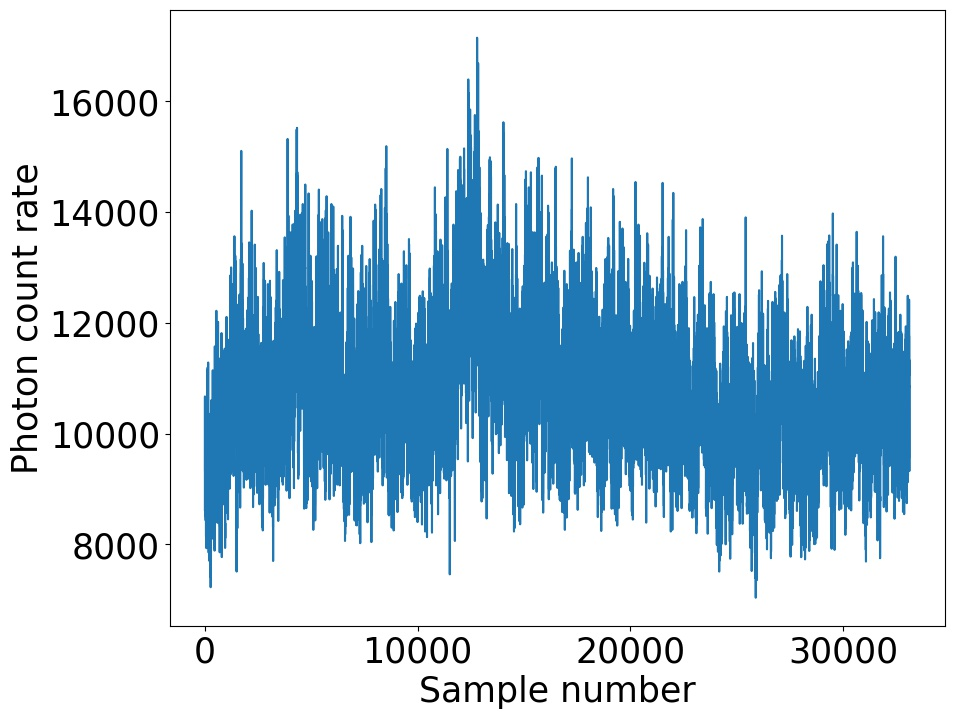
\includegraphics[width=0.9\linewidth]{sac_ascf_phi.jpg}
\caption{A representative stochastic time series of class $\phi$ of \textit{GRS 1915 + 105}. X-axis: Sample number (Scale: 0 - 35000), Y-axis: Photon count rate (Scale: 0 - 18000). }
\label{phi_ts}
\end{figure}

\begin{figure}[ht]
\centering
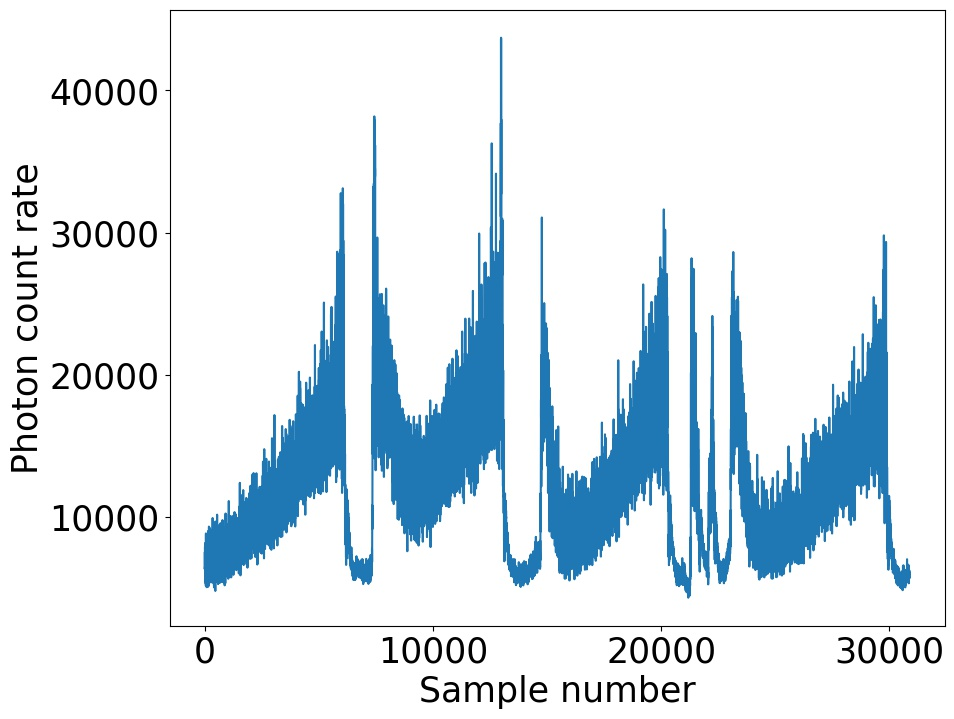
\includegraphics[width=0.9\linewidth]{sac_ascf_theta.jpg}
\caption{A representative non-stochastic time series of class $\theta$ of \textit{GRS 1915 + 105}. X-axis: Sample number (Scale: 0 - 35000), Y-axis: Photon count rate (Scale: 0 - 45000). }
\label{theta_ts}
\end{figure}

\section{Results and Discussion}

\subsection{Results of SVD based analysis}


%From SVD decomposition of the data matrix, we pick up the top 2 right singular vectors (E1, E2) corresponding to the temporal dynamics and plot E1 vs E2 for each time series. Figure \ref{svd_e1e2_nonstochastic} shows the panel of representative E1-E2 plots for time series  that are classified as non-stochastic and Figure \ref{svd_e1e2_stochastic}  shows the corresponding panels for time series that are classified as stochastic. The Betti number descriptors for each of the E1-E2 plots are tabulated in Table \ref{tab:results} under the column Betti descriptors. In order to infer the label of the time series from the Betti descriptors, We use the following strategy. Betti descriptor $\beta = (\beta_0, \beta_1)$. We use the L1-norm of $\beta$. If $\lvert \beta \rvert \gt 1$ then the time series is classified as non-stochastic else the time series is stochastic.

From SVD decomposition of the data matrix, we plot the top 2 right singular vectors (E1 vs E2) to understand the temporal dynamics for each time series. Figure \ref{svd_e1e2_nonstochastic} shows representative E1 vs E2 plots for time series  that are classified as non-stochastic and Figure \ref{svd_e1e2_stochastic}  shows the corresponding plots for time series that are classified as stochastic. The Betti number descriptors for each of the E1 vs E2 plots are tabulated in Table \ref{tab:results} under the column \textit{Betti descriptor}. In order to infer the label of the time series from the Betti descriptors, we use the L1-norm of $\beta$, $\|\beta\|_1$. If $\|\beta\|_1 > 1$, the time series is classified as non-stochastic, else the time series is stochastic.

%\begin{figure*}[ht]
% \centering
% \subfigure[] {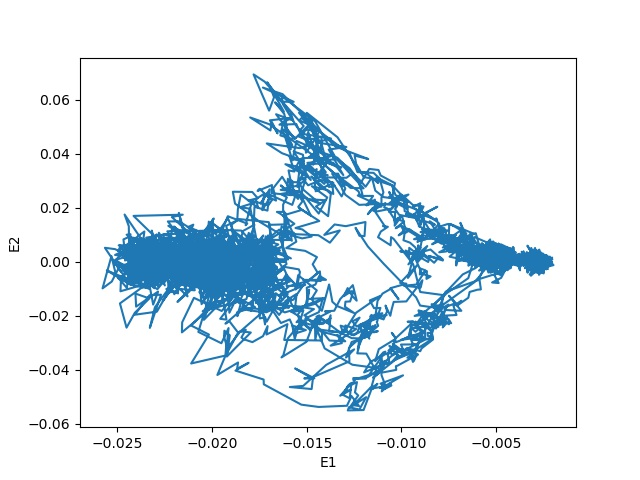
\includegraphics[width=-.3\linewidth]{sac_ascf_kappa_e1_vs_e2_m_2_tau_50.jpg}}
% \subfigure[] {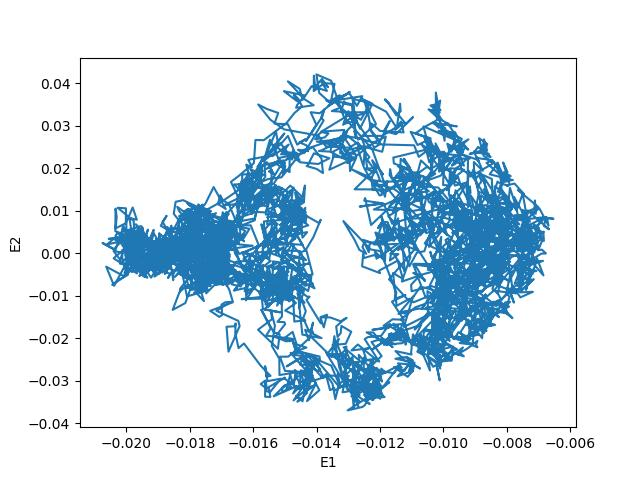
\includegraphics[width=-.3\linewidth]{mu_e1_vs_e2_m_4_tau_80.jpg}}
%  \subfigure[] {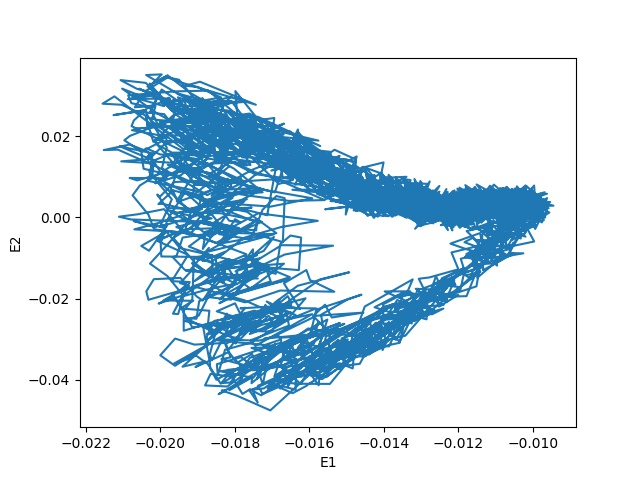
\includegraphics[width=-.3\linewidth]{rho_svd.jpg}}
% \caption{Plot of E1 vs E2 (top two right singular vectors) of data matrix for  representatives from non-stochastic time series of \textit{GRS 1915 + 105}. The series are $\kappa$, $\mu$ and $\rho$ from left to right.}
% \label{svd_e1e2_nonstochastic}
%\end{figure*}

\begin{figure*}
   \centering
   \subfigure[]{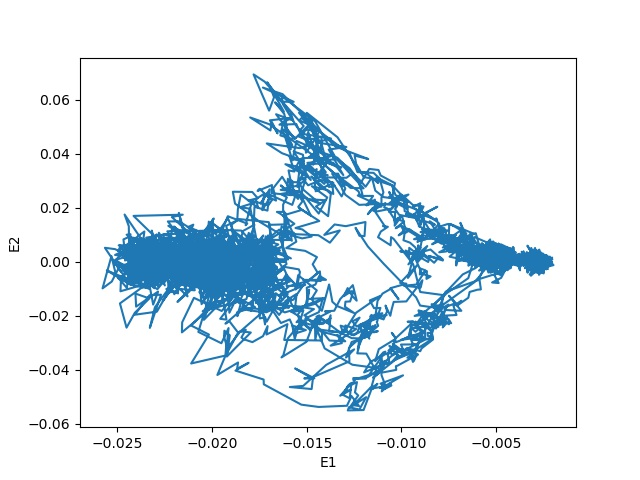
\includegraphics[width=0.28\textwidth]{sac_ascf_kappa_e1_vs_e2_m_2_tau_50.jpg}}
   \subfigure[]{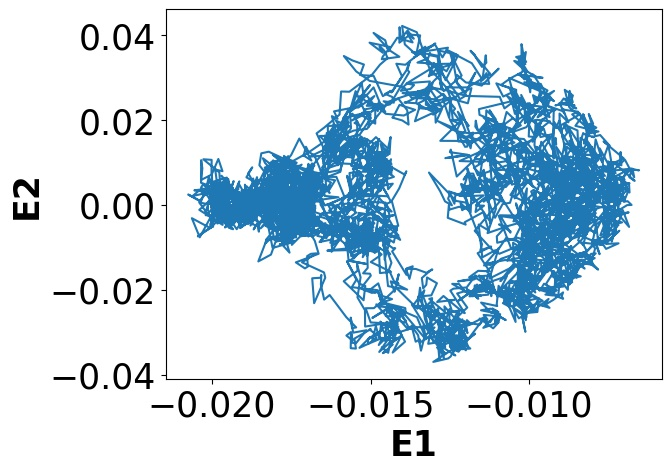
\includegraphics[width=0.28\textwidth]{sac_ascf_mu_e1_vs_e2_m_4_tau_80.jpg}}
   \subfigure[]{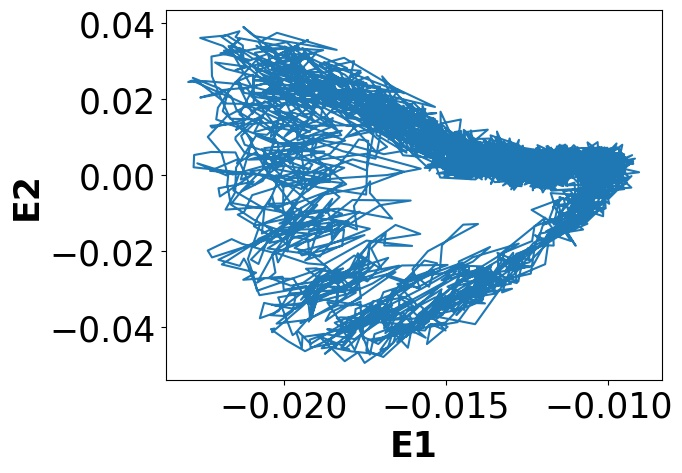
\includegraphics[width=0.28\textwidth]{sac_ascf_rho_e1_vs_e2_m_8_tau_20.jpg}}
   \caption{Plot of E1 vs E2 (top two right singular vectors) of data matrix for  representatives from non-stochastic time series of \textit{GRS 1915 + 105}. The series are $\kappa$, $\mu$ and $\rho$ from left to right.}
   \label{svd_e1e2_nonstochastic}
\end{figure*}

%\begin{figure*}[ht]
% \centering
% 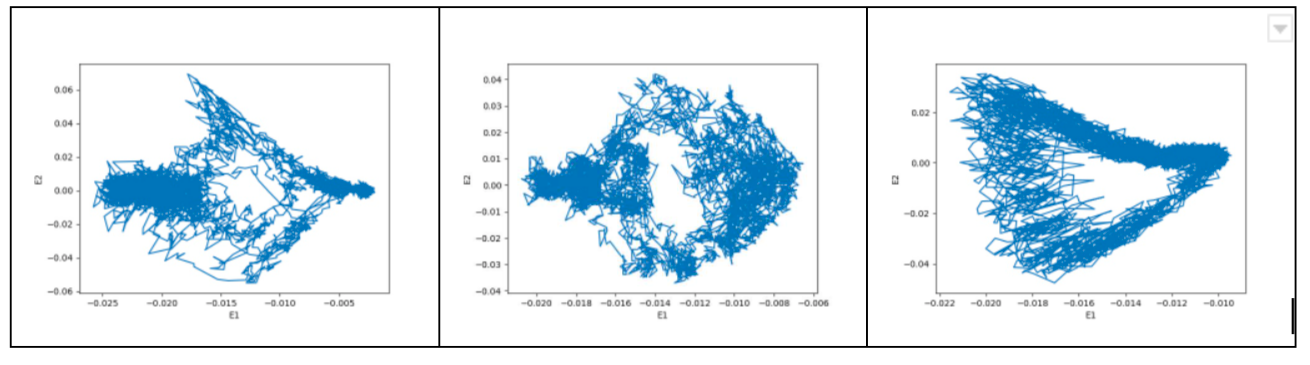
\includegraphics[width=\linewidth]{svd_non_stochastic.png}
% \caption{Plot of E1 vs E2 (top two right singular vectors) of data matrix for  representatives from non-stochastic time series of \textit{GRS 1915 + 105}. The series are $\kappa$, $\mu$ and $\rho$ from left to right.}
% \label{svd_e1e2_nonstochastic}
%\end{figure*}

\begin{figure*}
   \centering
   \subfigure[]{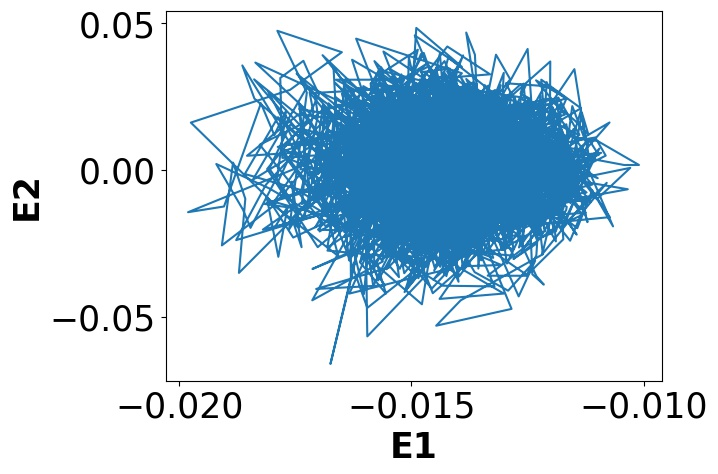
\includegraphics[width=0.28\textwidth]{phi_e1_vs_e2_m_2_tau_20_S.jpg}}
   \subfigure[]{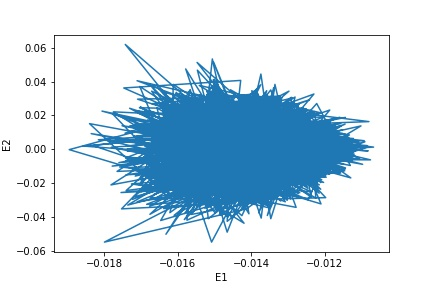
\includegraphics[width=0.28\textwidth]{khai_e1_vs_e2_m_2_S.jpg}}
   \subfigure[]{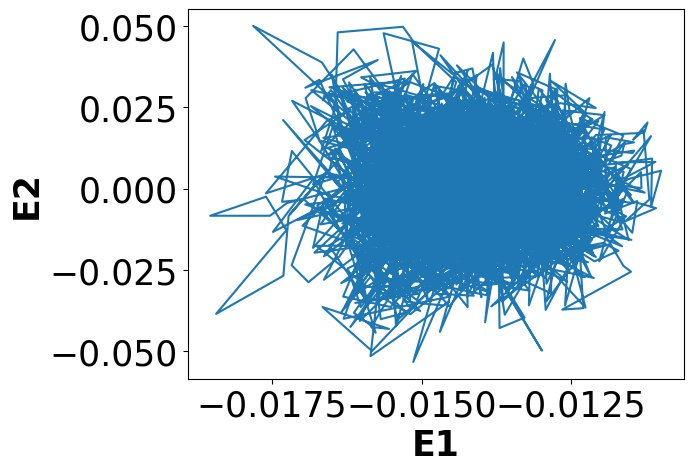
\includegraphics[width=0.28\textwidth]{gamma_e1_vs_e2_m_2_tau_20_S.jpg}}
\caption{Plot of E1 vs E2 (top two right singular vectors) of data matrix for  representatives from  stochastic time series  of \textit{GRS 1915 + 105}. The series are $\phi$, $\chi$ and $\gamma$ from left to right.}
   \label{svd_e1e2_stochastic}
\end{figure*}


\subsection{Results of PCA based analysis}

\begin{figure}[ht]
\centering
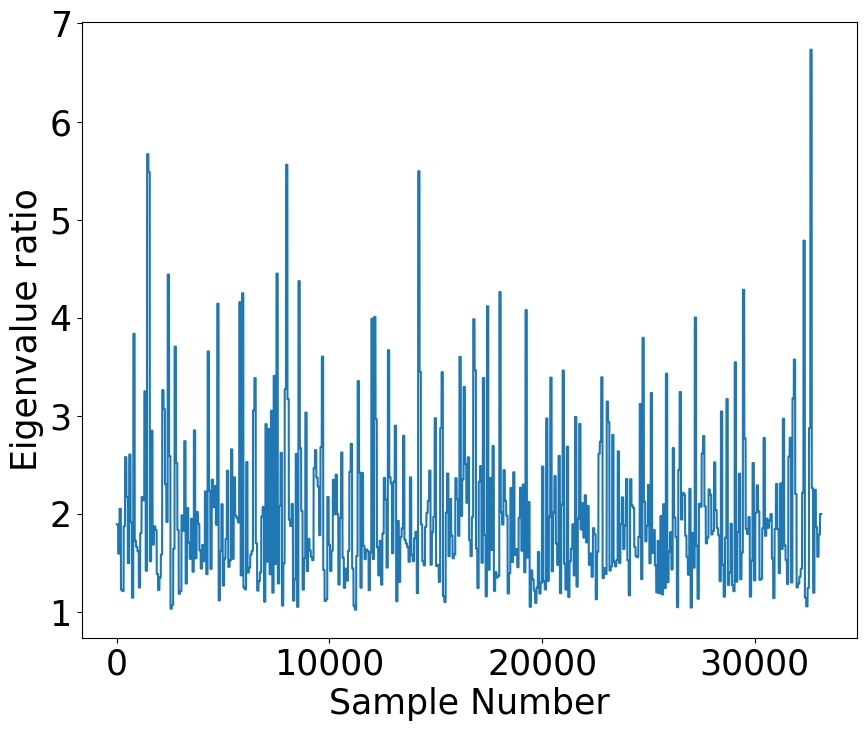
\includegraphics[width=1\linewidth]{sac_ascf_phi_eig.jpg}
\caption{Plot of eigenvalue ratio of the stochastic time series shown in Figure \ref{phi_ts}. X-axis: Sample number (Scale: 0 - 35000), Y-axis: Eigenvalue ratio (scale- 0 - 7). MER=7}
\label{phi_eig}
\end{figure}

\begin{figure}[ht]
\centering
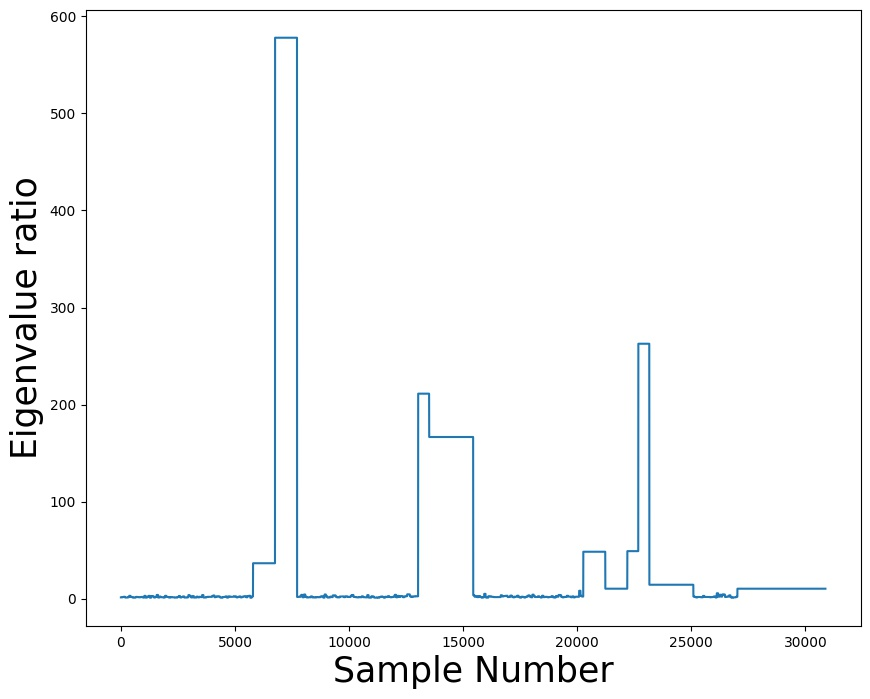
\includegraphics[width=1\linewidth]{sac_ascf_theta_eig.jpg}
\caption{Plot of eigenvalue ratio of the  non-stochastic time series shown in Figure \ref{theta_ts}. X-axis: Sample number (Scale: 0 - 35000), Y-axis: Eigenvalue ratio (scale- 0 - 600). MER=577 }
\label{theta_eig}
\end{figure}

Figures \ref{phi_eig} and \ref{theta_eig} show the eigenvalue ratio plots for stochastic time series shown in Figure \ref{phi_ts} and  non-stochastic time series shown in Figure \ref{theta_ts} respectively. We compute the three PCA based features which are MER, VAR and Area  and utilize them for classification using the following observations:

\begin{itemize}
\item MER: For stochastic time series, eigenvalue ratios  are small across the entire time series, typically lying in the range 1-20. This implies that MER  will also be small. On the other hand, for  non-stochastic time series the eigenvalue ratios are significantly high, typically reaching a few hundreds in certain sub-intervals. Hence the MER for a non-stochastic time series is typically large.
\item VAR: For a stochastic signal since the range of eigenvalue ratios is typically small, the VAR is also small. On the other hand, for a non-stochastic signal, since the eigenvalue ratios occupy a large range of values, VAR is typically high.
\item Area: For a stochastic time series, since the eigenvalue ratios  are small the Area is also small. However, for a non-stochastic signal the eigenvalue ratios remain high for longer time intervals. Hence the Area is significantly higher.
\end{itemize}

\subsection{Consolidated Results}

Table \ref{tab:results}  tabulates the computed features and the respective inferences using the proposed approaches. Comparison of our results with CI based approach \cite{Adegoke2018} is also presented. The columns of the table are described below.

\begin{enumerate}
\item Column 1 (\textit{Class}) gives the class of the time series \cite{Adegoke2018}.
\item Column 2 (\textit{diskbb}) and column 3 (\textit{PL}) give quantities diskbb and  PL, respectively, which indicate the spectral states of the black hole \cite{Adegoke2018}.
\item Column 4 (CI Inference) gives the inference about the state of the time series using CI approach \cite{Adegoke2018}.
\item Column 5 (Betti descriptor) gives the Betti description of the E1 vs E2 plots and column 6 gives the SVD based inference.
\item The computed PCA based features: MER, VAR and Area  are tabulated in columns 7, 8 and 9 respectively. Our inference using these PCA features is given in column 10.
\item Finally the last column gives if there is a match between all three inferences.
\end{enumerate}


\begin{table*}[t]
\caption{Timeseries: Comparison between CI based label and inference using proposed approaches. The mismatched time series class, $\delta$, is shown in bold. (LC stands for Limit Cycle \cite{Adegoke2018} which is non-stochastic, $F$ stands for Fractal which is also non-stochastic and $S$ stands for stochastic)}
\begin{center}
\begin{tabular}{|p{0.5cm}|p{0.75cm}|p{0.75cm}|p{1cm}|p{2.5cm}|p{3cm}|p{0.75cm}|p{1cm}|p{0.5cm}|p{1.8cm}|p{0.75cm}|}
\hline
Class & diskbb & PL  & CI \newline Inference & Betti descriptor & SVD  \newline Inference & MER & Variance & Area & PCA \newline Inference  &  Match \\
\hline
$\beta$ & 46 & 52 & F & (1,3) & Non-stochastic & 214 & 483 & 43 & Non-stochastic & Yes\\
\hline
$\theta$  & 11 &  88 & F & (3, 2) & Non-stochastic & 577 & 778 & 58&Non-stochastic  &  Yes \\
\hline
$\lambda$ &  54 & 46 & F & (1,3) & Non-stochastic & 600 & 6782 & 314 & Non-stochastic & Yes \\
\hline
$\kappa$ &  59 & 51 & F & (1,2) & Non-stochastic & 700 & 5199 & 144 & Non-stochastic &  Yes \\
\hline
$\mu$  & 56 & 41 & F & (1,1) & Non-stochastic & 50 & 51 & 12 & Non-stochastic & Yes \\
\hline
$\nu$  & 28 & 72 & F & (1,6) & Non-stochastic & 30 & 32 & 16 & Non-stochastic & Yes\\
\hline
$\alpha$  & 23 & 77& F & (6,0 ) & Non-stochastic & 30 & 1.9 & 27.7 & Non-stochastic & Yes \\
\hline
$\rho$  & 28 & 72 & LC & (1,1) &  Non-stochastic & 60 & 147 & 35 & Non-stochastic & Yes \\
\hline
\textbf{$\delta$}  & \textbf{48} & \textbf{50} &  \textbf{S} & \textbf{(1,0)}& \textbf{Stochastic}& \textbf{42} & \textbf{9.74} & \textbf{26.2} & \textbf{Non-stochastic} &  \textbf{No} \\
\hline
$\phi$  & 50 & 34 & S & (1,0)& Stochastic & 7 & 0.5 & 15 & Stochastic &  Yes \\
\hline
$\gamma$  & 60 & 31 & S & (1,0)& Stochastic & 12 & 1 & 16 & stochastic &  Yes \\
\hline
$\chi$  & 09 & 89 & S & (1,0)& Stochastic & 5.6 & 0.25 & 6.05 & Stochastic &  Yes \\
\hline
\end{tabular}
\label{tab:results}
\end{center}
\end{table*}

\begin{figure}
  \centering
  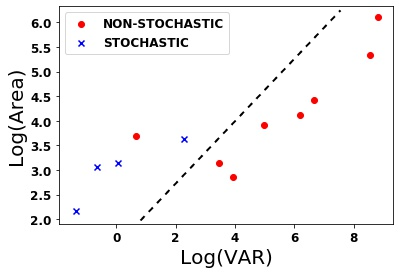
\includegraphics[width=.9\linewidth]{variance_area.drawio.png}
  \caption{Feature space (VAR and Area) shows that the two classes are well separated. The dashed line shows the decision boundary separating the two classes. The label of one of the time series is ambiguous.}
  \label{fig:variance_area_fs}
\end{figure}
We observe that SVD based analysis results in classification  is consistent with CI based results for all the 12 classes of time series. However, with PCA based approach the inference for  $\delta$ time series is not consistent with other two approaches. We observe that the PCA based features, VAR and Area, result in visible clustering as shown in Figure \ref{fig:variance_area_fs}. This could be attributed to the fact that   these features take into account the entire span of time series and hence form robust feature space. According to the CI based analysis $\delta$ turns out to be in between states slim disc  and GAAF \cite{Adegoke2018}. However, the present analysis shows that $\delta$ falls in between ADAF and Keplerian disc.


\section{Conclusion}
Exploring different techniques in order to have a conclusive inference for black hole systems turns out to be indispensable. We explore two different classical matrix based techniques to identify states of \textit{GRS 1915+105} black hole using the time series obtained from \textit{RXTE} satellite data. Based on our analysis, we are able to identify two extreme temporal dynamical classes of accretion around black holes. In the first approach we extend  SVD decomposition to understand temporal dynamics,  by adding  topological descriptors, to classify time series as stochastic vs non-stochastic. In yet another approach, a novel application of  PCA  to characterize the time series is proposed. We compare inferences of the CI based approach with those obtained using the proposed matrix based methods. Of the 12 classes of time series analysed, a mismatch is observed in the PCA based inference of only one class, while all other classes concur.

\begin{thebibliography}{1}

\bibitem{Belloni2000}
Belloni, T., et al. ``A model-independent analysis of the variability of GRS 1915+ 105." arXiv preprint astro-ph/0001103 (2000).

\bibitem{Mukhopadhyay2004}
Mukhopadhyay, Banibrata. ``Chaotic behavior of micro quasar GRS 1915+ 105." AIP Conference Proceedings. Vol. 714. No. 1. American Institute of Physics, 2004.

\bibitem{misra2006}
Misra, Ranjeev, et al. ``The nonlinear behavior of the black hole system grs 1915+ 105." The Astrophysical Journal 643.2 (2006): 1114.

\bibitem{Shakura1973}
Shakura, Ni I., and Rashid Alievich Sunyaev. ``Black holes in binary systems. Observational appearance." Astronomy and Astrophysics 24 (1973): 337-355.

\bibitem{chakrabarti1995}
Chakrabarti, Sandip K., and Lev G. Titarchuk. ``Spectral properties of accretion disks around galactic and extragalactic black holes." arXiv preprint astro-ph/9510005 (1995).

\bibitem{narayan1994}
Narayan, Ramesh, and Insu Yi. ``Advection-dominated accretion: Underfed black holes and neutron stars." arXiv preprint astro-ph/9411059 (1994).

\bibitem{Adegoke2018}
Adegoke, Oluwashina, et al. ``Correlating non-linear properties with spectral states of RXTE data: possible observational evidences for four different accretion modes around compact objects." Monthly Notices of the Royal Astronomical Society 476.2 (2018): 1581-1595.

\bibitem{Abramowicz1988}
Abramowicz, M. A., et al. ``Slim accretion disks." The Astrophysical Journal 332 (1988): 646-658.

\bibitem{rajesh2010}
Rajesh, S. R., and Banibrata Mukhopadhyay. ``Two-temperature accretion around rotating black holes: a description of the general advective flow paradigm in the presence of various cooling processes to explain low to high luminous sources." Monthly Notices of the Royal Astronomical Society 402.2 (2010): 961-984.

\bibitem{jmlr}
Naitzat, Gregory, Andrey Zhitnikov, and Lek-Heng Lim. ``Topology of Deep Neural Networks." J. Mach. Learn. Res. 21.184 (2020): 1-40.

\bibitem{Bandt2002}
Bandt, Christoph, and Bernd Pompe. ``Permutation entropy: a natural complexity measure for time series." Physical review letters 88.17 (2002): 174102.

\bibitem{Boaretto2021}
Boaretto, B. R. R., et al. ``Discriminating chaotic and stochastic time series using permutation entropy and artificial neural networks." Scientific reports 11.1 (2021): 1-10.

\bibitem{lacasa2010}
Lacasa, Lucas, and Raul Toral. ``Description of stochastic and chaotic series using visibility graphs." Physical Review E 82.3 (2010): 036120.

\bibitem{Brunton2016}
Brunton, Steven L., Joshua L. Proctor, and J. Nathan Kutz. ``Discovering governing equations from data by sparse identification of nonlinear dynamical systems." Proceedings of the national academy of sciences 113.15 (2016): 3932-3937.

\bibitem{xte}
 RXTE Public Data \url{https://heasarc.gsfc.nasa.gov/docs/xte/xte_public.html}

\end{thebibliography}

%https://heasarc.gsfc.nasa.gov/docs/xte/XTE.html
%https://heasarc.gsfc.nasa.gov/docs/xte/xte_public.html


\end{document}

